% !TEX root = ../../thesis.tex


\chapter{Drittes Kapitel}\label{ch:drittes_kapitel}

Ich leite das Kapitel ein!

\begin{figure}[H]
    \centering
    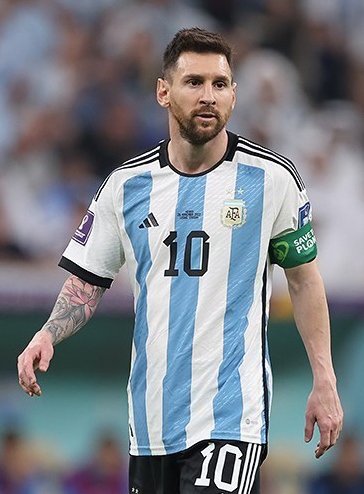
\includegraphics[width=0.5\textwidth]{contents/03_Drittes_Kapitel/Messi}
    \caption{Das ist Lionel Messi}
    \label{fig:messi_1}
\end{figure}

\begin{figure}[H]
    \centering

    \begin{subfigure}{0.5\textwidth}
        \centering
        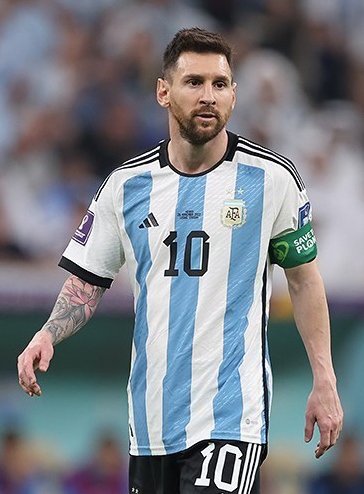
\includegraphics[width=0.8\textwidth]{contents/03_Drittes_Kapitel/Messi}
        \caption{Links}
        \label{fig:messi_2_1}
    \end{subfigure}%
    \begin{subfigure}{0.5\textwidth}
        \centering
        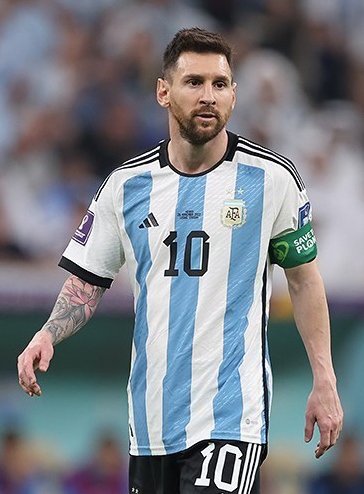
\includegraphics[width=0.8\textwidth]{contents/03_Drittes_Kapitel/Messi}
        \caption{Rechts}
        \label{fig:messi_2_2}
    \end{subfigure}
    \caption{Gesamt-Bildbeschreibung}
    \label{fig:messi_2}
\end{figure}

% Einbinden von anderen Dateien, damit diese Datei hier nicht riesig wird
% !TEX root = ../../thesis.tex


\section{Abschnitt 1}\label{sec:abschnitt_1}

Ich bin eine Tabelle:

\begin{table}[H]
    \begin{center}
        % c für "center" (alternativ "l" oder "r")
        % Die | geben die Linien der Tabelle an -> außen einfache, innen doppelte Linien
        \begin{tabular}{|c || c|}
            \hline
            \textbf{Überschrift 1} & \textbf{Überschrift 2} \\
            \hline
            \hline
            A                      & a                      \\
            \hline
            B                      & b                      \\
            \hline
        \end{tabular}
        \caption{Tabellenbeschreibung}
        \label{tab:table_1}
    \end{center}
\end{table}

% !TEX root = ../../thesis.tex


\section{Abschnitt 3}\label{sec:abschnitt_3}

Ich bin eine Aufzählung \textit{ohne} Nummerierung:

\begin{itemize}
    \item Erster Stichpunkt
    \item Zweiter Stichpunkt
    \item Dritter Stichpunkt
\end{itemize}

% Nach Aufzählungen wird die erste Zeile danach etwas eingerückt.
% Wenn man das nicht möchte, kann man \noindent verwenden.
\noindent Ich bin eine Aufzählung \textit{mit} Nummerierung:

\begin{enumerate}
    \item Erster Stichpunkt
    \item Zweiter Stichpunkt
    \item Dritter Stichpunkt
\end{enumerate}

% !TEX root = ../../thesis.tex


\section{Abschnitt 4}\label{sec:abschnitt_4}

Ich bin eine mathematische Formel:

\[e^{\pi * i} = -1\]
\[a = \frac{F}{m}\]
\[\sum_{i = 1}^n i = \frac{n(n + 1)}{2}\]

Letztere Formel ist die Gaußsche Summenformel\footnote{Benannt nach Carl Friedrich Gauß}.

% !TEX root = ../../thesis.tex


\section{Abschnitt 5}\label{sec:abschnitt_5}

Hier kann ich diverse Sachen referenzieren:

\begin{itemize}
    \item Kapitel~\ref{ch:einleitung} und Anhang~\ref{ch:erster_anhang}
    \item Abschnitt~\ref{sec:test_abschnitt} und Unterabschnitt~\ref{subsec:test_unterabschnitt}
    \item Paragraph~\ref{par:test_paragraph_1}
    \item Bilder, wie zum Beispiel Abb.~\ref{fig:messi_2_1}
\end{itemize}

Es können nur Sachen referenziert werden, die ein entsprechendes label-Tag verwenden.


\pagebreak
